\documentclass{IEEEtran}

\usepackage[utf8]{inputenc}
\usepackage{graphicx}
\usepackage[spanish]{babel}
\usepackage{authblk}

\begin{document}

	\title{Sistema de monitoreo de lactantes durante el sueño para la disminución del riesgo del síndrome de muerte súbita}
	\author{Autor: Diego Ariel Bertolini}
	\affil{Tutor: Filippo Visco Comandini}
	\affil{Facultad de Ingeniería, Universidad de Palermo}
	\date{Mayo de 2018}	
	\maketitle

	%Key references
	%Sistema, monitor, alerta, bebé, lactante, síndrome de muerte súbita, sueño
	
	\begin{abstract}
		El presente proyecto de investigación se enfoca en la realización de un dispositivo que realice la tarea de monitorear a un bebé durante las horas de sueño a través de distintos sensores incorporados a una cuna o sector donde descansa el lactante. 

		Los sensores incorporados en el dispositivo permitirían controlar la respiración, movimiento, humedad, temperatura ambiente y corporal, para evitar así la gran problemática de las muertes súbitas durante el sueño.
		
		El sistema general incorporaría una forma de alerta hacia los padres o tutores ante la detección de variaciones drásticas en los distintos indicadores de datos que se toman desde los sensores y serán visualizados a través de una aplicación móvil instalada en los dispositivos de los tutores.
	\end{abstract}
	
	\section{Introducción}
	
%Introduccion
%	Idea
%	Estructura

		\fontfamily{pcr}
	
		El síndrome de muerte súbita en el lactante \textbf{(SMSL)} se define como la muerte repentina, inesperada y sorpresiva de un niño generalmente menor de un año de edad, que si bien la muerte súbita no es exclusiva del lactante ya que puede presentarse en niños mayores, jóvenes y adultos, pero en la mayoría de los casos se da en el lactante y es hacia ese enfoque en donde se desarrolla el presente trabajo de investigación. 

		Gran parte de los padres primerizos enfrentan con mucho temor los primeros meses de vida de un hijo, pues es en esa época en donde se presentan situaciones desesperantes en el cuidado del recién nacido con el conocido síndrome de muerte súbita, y en el caso de que ocurriera, ésta resultaría ser una situación realmente desgarradora en donde muy pocas familias están preparados para afrontar este hecho.

		A través de los años se ha avanzado de manera contundente en el estudio sobre el conocido síndrome de muertes súbitas en lactantes con pocos días de vida. Ésto permitió desarrollar una serie de medidas y dispositivos que permitirían la reducción significativa del número de muertes producidas por dicha problemática. Según distintos índices publicados en distintos paper y que fueron recolectados durante años, se puede observar la disminución de dichos indicadores gracias a acciones tomadas en cuenta o tratamientos según antecedentes detectados. 

		Existen distintos factores que han sido estudiados según casos precedentes y destacados en el asunto a ser sociales, maternos y perinatales que están altamente relacionados con el SMSL. Los factores sociales son los más significativos en lo que hace referencia a las sociedades con un pobre nivel educacional y económico, siendo causante de un importante número de muertes causadas dentro de dichas circunstancias. Los factores maternos tiene que ver con la edad de la madre, que al ser inferior a unos 20 años existe un menor cuidado y tiempos intergenésicos más acotados, lo cual es considerado como un riesgo para el lactante. Los factores perinatales hacen referencia a los siguientes indicadores y características a ser:
	
		\begin{itemize}
			\item Peso de nacimiento \textless 2.500 gramos - OR: 9.3 (5,1 - 17)
			\item Edad gestacional \textless 38 semanas - OR: 5,7 (3,5 - 9,8)
			\item Retraso del crecimiento intrauterino (\textless 10º percentilo) - OR: 3,1 (2,0 - 4,9)
			\item Madre soltera - OR: 2,9 (1,7 - 5,0)
			\item Partos múltiples - OR: 8,7 (3,41 - 20,05)
			\item Admisión en terapia intensiva neonatal - OR: 4,25 (2,91 - 6,21)
		\end{itemize}

		\subsection{Historia}

			En la antigüedad se desconocían cuáles eran los factores principales que causaban el SMSL, hasta en muchos casos se le atribuían ciertas creencias religiosas por la ocurrencia de semejante tragedia, que hoy en día puedría llegar a verse reflejado por las diferentes culturas existentes a lo largo y ancho del mundo. Incluso décadas atrás se hacía muy dificil tomar estadísticas basadas en casos puntuales y así desarrollar predicciones que pudieran llevar a desencadenar semejante tragedia, por consiguiente y sin estudios fundados, los padres o tutores de los lactantes llegaban a tomar ciertas medidas para controlarlos de manera más cercana y evitar tragedias, pudiendo ser o no de ayuda, pero en una gran cantidad de casos sin saber que pudieran estar contribuyento a esta gran problemática.

			En la \textbf{Figura \ref{tablahistoria}} se representa en una tabla comparativa de indicadores referidos a mortalidad por el síndrome de muerte súbita en el lactante durante los años 1991 y 1998, diferenciadas por distintas categorías destacadas.

			\begin{figure}
				\centering
				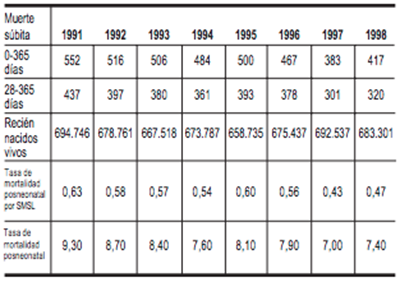
\includegraphics[width=1\linewidth]{tablahistoria}
				\caption{Tabla comparativa 1991-1998}
				\label{tablahistoria}
			\end{figure}

			Transcurrido un tiempo y habiendo realizado estudios contundentes sobre el síndrome en cuestión, se lograron obtener ciertos factores determinantes para estudiar probabilidades y así concientizar sobre métodos de prevención o mecanísmos fisiopatológicos. 

		\subsection{Epidemología}

			Ciertos aspectos epidemológicos resultan interesantes a ser analizados. En los países desarrollados era donde mayor cantidad de SMSL se detectaban. En Estados Unidos, hasta antes del año 1992, se observaba un índice de 1,2 fallecidos por mil nacidos vivos, pero de allí en adelante ha decendido notablemente siendo en 2001 de 0,56 por mil nacidos vivos, lo cual representa una disminución del 53\% registrada en un transcurso de 10 años. Por otra parte, en los países subdesarrollados, se plantea un esquema estadístico un poco más complejo ya que existen grandes variaciones dependiendo de diferencias étnicas, raciales, hábitos, constumbres, ambiente socioeconómico y cultural, factores sociales, psicológicos y médicos, etc. En éstos casos, la mayor incidencia recide en los niños lactantes de 2 a 4 meses de vida, durante los meses de invierno y en horario nocturno de 12 AM a 6 AM, siendo el sexo masculino el más afectado.

			\begin{figure}
				\centering
				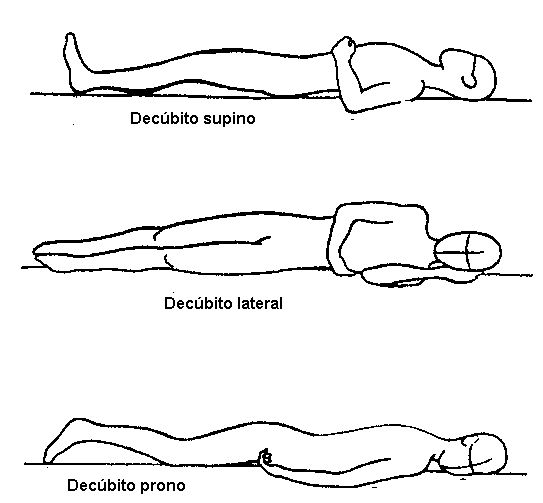
\includegraphics[width=1\linewidth]{posiciones}
				\caption{Diferentes posiciones}
				\label{posiciones}
			\end{figure}

			Ante la propuesta de diferentes posiciones en las que se debe colocar el lactante para dormir, se ha especulado con una gran cantidad de opiniones y conjeturas sobre las mismas, dando lugar la gran pregunta que toda madre se quiere hacer: "¿Qué posición es realmente la indicada para que duerma el bebé?". El estudio de distintas posiciones de colocación del lactante al momento de dormir ha permitido obtener ciertos indicios que pudieran llegar a minimizar el riesgo del SMSL ya que esta estrechamente relacionado con las posiciones en las cuales se encuentra la traquea y laringe las cuales influyen directamente con la respiración. En países donde hace muchos años se recomienda la posición supina, no ha ocurrido un aumento de muertes de niños atribuibles por aspiración, por ejemplo en el Reino Unido, Nueva Zelanda, entre otros.

			Se han detectado que en las épocas de mayor temperatura y el niño durmiendo en una posición de prona (como muestra la \textbf{Figura \ref{posiciones}} pero para lactantes), el riesgo de SMSL aumenta, y en el caso de que haya antecedentes de infecciones en las vías respiratorias aumenta aún más las probabilidades. Lo cierto es que la posición en la cual se posiciona el lactante para dormir es muy importante ya que está atado a ciertos factores como por ejemplo la del reflujo gastroesofárico en caso de vómito, o mismo movimiento nocturno y que ambas amenazas pudiera llegar a ocacionar una obtrucción en las vías respiratorias.

		\subsection{Estudios realizados en víctimas del SMSL}

			Ante aquellos trágicos y lamentables casos en donde ha ocurrido éste síndrome, se han realizado distintos análisis e inspecciones con los que se puede obtener ciertas conclusiones o motivos por los cuales ocurrió el mismo. En algunos casos la muerte súbita recide en algún historial o causante ya conocido y diagnosticado previamente por ejemplo problemas del metabolismo, algunas cardiopatías congénitas, traumatísmos, anomalías del sistema nervioso central, etc., en los cuales no se va a enfocar la presente investigación. En los otros casos en los cuales la presente investigación sí va a hacer incapié se basa en casos donde no se han identificado malos cuidados o falta de nutrición e hidratación, o incluso antecedentes clínicos, sino en los casos en los que por ejemplo las causas de muerte se han detectado por el hallazgo de líquidos blanquecinos en las cavidades pulmonares o vías respiratorias superiores compatibles con leche, por lo que se determina el fallecimiento por asfixia causada por vómitos, apnea, o casos de movimiento nocturno que comprometen en la respiración del lactante ocacionando otra forma de asfixia.
		
		\subsection{Recomendaciones para evitar el SMSL}

			Distintas estrategias se han desarrollado con el fin de disminuir al máximo el riesgo a contraer tal síntoma, basadas en recomendaciones desarrolladas por grupos médicos y científicos que estudiaron con profundidad el caso. Cabe destacar que a medida que pasó el tiempo algunas características que serán mencionadas a continuacion han sufrido cambios, los cuales se vieron modificados por actualización de distintos métodos según el paso del tiempo y nuevas costumbres y hasta tecnologías.

			Las recomendaciones que se mencionan a continuación son un estracto puntual de algunos pocos años atrás, a ser:

			\begin{itemize}
				\item Posición de colocación del bebé supina para dormir.
				\item El espacio donde duerme debe tener ciertas medidas de seguridad en cuanto a los productos utilizados y sus materiales.
				\item Superficie del lugar donde duerme debe ser acorde al lactante (no debe ser colchones de agua o superficies blandas).
				\item Evitar el uso de productos blandos para almohadas, frazadas o juguetes.
				\item Evitar el sobrecalentamiento.
				\item Evitar el colecho.
			\end{itemize}

	\section{Casos de estudio}

		En ésta sección se mencionan los aspectos principales a ser estudiados dentro del entorno en el cual se desarrolla la actividad diaria en cada hogar con respecto al área donde descansa el bebé, para así obtener datos específicos y reducir riesgos. Las áreas de estudio son:

		\begin{itemize}
			\item Cuna donde descansa el bebé
			\item Posicionamiento del lactante dentro del área de estudio
			\item Temperatura corporal
			\item Respiración
			\item Movimientos
		\end{itemize}

		El cuidado de bebés durante las horas de sueño es un proceso altamente demandante y estresante en tiempo para las personas a cargo. La tarea incluye el control de ciertos factores que determinan el bien estar del bebé y el análisis de disminución de riesgos ante tragedias de muerte súbita durante ese proceso. En el ambiente en el que se encuentra existen variables como la luz, temperatura, humedad, ruido e incluso la calidad del aire o la ausencia de determinados gases que pueden ser dañinos para un bebé. El objetivo del presente proyecto es analizar datos obtenidos por los sensores dentro del ambiente en el cuál se van a enfocar en el movimiento, respiración y temperatura del bebé, para así identificar emergencias que pueden ser causadas por episodios que desencadenen en una muerte súbita por obstrucción de las vías respiratorias, ante los cámbios drásticos de los indicadores o variables ambientales.
		
		El proyecto se focaliza en realizar el control de estas variables, facilitando la tarea de las personas a cargo en cuando al control que realizan noche tras noche y ofreciendo mayor tranquilidad en el cuidado. Esta tecnología nos permite identificar episodios en los cuales comprometen la salud del bebé ya sea por movimientos que puedan generar una obtrucción en las vías respiratorias, vómitos durante la noche y en una posición comprometida, posibles casos epilépticos con un exceso de movimiento, para finalmente notificar a las personas encargadas del cuidado del lactante y tomar medidas inmediatas.

		\subsection{Cuna o área analizada}

		Desde su nacimiento hasta algunos meses despues, los bebés tienen los músculos poco desarrollados como para poder evitar posiciones o incidentes indeseados que generen descenlaces dramáticos. La cuna es el principal lugar donde el bebé descansa y pasa la mayor parte del día, y en donde los padres o tutores pierden la atención mayor cantidad del tiempo sobre todo por las noches. A través del tiempo se hicieron cambios en el diseño de las cunas para mejorar la calidad de vida de los pequeños, ya sea haciéndolas más ergonómicas, previniendo malas posturas y hasta utilizando ingeniería en materiales para evitar el desarrollo de agentes biológicos que pueden ser dañinos para seres humanos sin un sistema inmunológico completamente desarrollado. La utilización de materiales indicados en la construcción de una cuna son altamente demandados, al igual que pinturas y adornos no tóxicos, ya que es inevitable que un bebe ocasionalmente se lleve a la boca y muerda lo que tiene a su alcance. Siguiendo estos lineamientos de cuidado para los recién nacidos, este proyecto realiza la implementación de un sistema de sensores a estas cunas, sin entrar en contacto directo con el bebé.
		
		\subsection{Posicionamiento dentro del área de estudio}

		La idea principal de éste análisis es el de determinar si el cuerpo del bebé se encuentra dentro de la zona de estudio, de manera tal de determinar si el sistema está en condiciones de realizar los monitoreos pertinentes o bien notificar hacia las personas responsables sobre el incidente detectado, que pudiera ser causado o no por el movimiento del lactante en un desplazamiento sobre la cuna. La funcionalidad sobre la detección del bebé dentro de la zona de estudio se basa en la habilitación de los sensores correspondientes para la toma de información, es decir que si el sistema detecta la ausencia del lactante, los indicadores recolectados tanto de temperatura o movimiento estarían fallando en los datos sensoreados, por lo tanto dichos indicadores deberían ser descartados.
		
		\subsection{Temperatura corporal}

		La temperatura del bebé debe ser controlada, no solo por cuestiones de determinar o ayudar a la toma de estadísticas que hagan al disparo de alertas por problemas, como también para llevar un control períodico. De ésta forma los tutores, padres o responsables pudieran llegar a analizar a lo largo del tiempo, por datos almacenados en un período de tiempo, la fluctuación de los valores, detectar si existe una elevación de su temperatura para detectar fiebres, o incluso la perdida del calor corporal por otras causas.

		\subsection{Respiración}

		La respiración es uno de los factores o indicadores principales en los cuales se va a enfocar este sistema. Uno de los principales problemas que causan el SMSL son causados por los movimientos nocturnos que dejan mal posicionados al bebé generando una obtrucción en las vias respiratorias. De misma manera ocurre en otras incidencias causadas por vómitos nocturnos con el bebé posicionado en una forma desfavorable para le expulsión completa de los líquidos segregados, causando así también una obstrucción en las vias respiratorias.

		La idea es que mediante ciertos sensores incorporados en el lugar de la conciliación del sueño se pueda detectar la constante vibración causada por los movimientos de respiración del lactante. La necesidad de contar con sensores altamente sensibles es indispensable para la detección satisfactoria de la vibración causada por la respiración sobre la superficie donde duerme el lactante. A lo largo de la investigación de éste trabajo se han encontrado diferentes proyectos que contemplan el análisis de estos parámetros de entrada, desde plataformas posicionadas por debajo del bebé, hasta dispositivos colocados en prendas de vestir o cinturones colocados en el abdomen. Una de las formas que se van a implementar para el presente trabajo de investigación reside en una plataforma que está posicionada debajo del lactante, de forma tal de tomar los indicadores o mediciones requeridas de la manera menos invasiva y natural posible.

		También es importante destacar que ante la lectura del posicionamiento del bebé dentro del área de estudio, éste indicador podría estar arrojando un valor nulo, o dicho con otras palabras, indicando como si no estuviera detectando respiración del bebé, es por ello que es importante la detección del cuerpo dentro del area de estudio y en tal caso descartar la información sensoreada.
	
		\subsection{Movimientos}

		Uno de los objetivos principales del proyecto es el de monitorear el movimiento del bebé cuando está recostado sobre su cuna o el lugar indicado para conciliar el sueño. El objetivo recide en analizar si el movimiento es alto a tal punto de considerar si es conveniente realizar un analisis exaustivo del sueño referido al movimiento, siendo éste un indicador a modo informativo para comportamientos. El movimiento puede detectarse de forma activa o pasiva. Cuando un sensor emite algún tipo de energía se trata de una detección activa, mientras que cuando el sensor no emite ningún tipo de energía, se trata de una detección pasiva.

	\section{Marco teórico}

		La presente sección tiene como objetivo principale mencionar cuáles son los ítem principales y fundamentales que entran en funcionamiento para la resolución de la problemática. Los distintos módulos corresponden a una serie de herramientas y posteriores desarrollos que harán al funcionamiento del sistema en su totalidad y visualización hacia el usuario final. Los ítems tratados son:

		\begin{itemize}
			\item Plaqueta Arduino
			\item Sensores
			\item Módulo de conectividad
			\item Aplicación para dispositivos móviles
		\end{itemize}

		\subsection{Esquema general}

			El marco general del sistema a implementar está comprendido por un hardware constituído por una plaqueta Arduino y sus sensores correspondientes para tomar los indicadores necesarios conectados a la plaqueta Arduino principal para procesar toda la información, y una aplicación móvil, instalada en un dispositivo como un teléfono celular o tablet, en donde se visualiza la información recolectada y arrojar alertas si corresponde. La conectividad entre la plaqueta Arduino y la aplicación móvil se realiza mediante un módulo Bluetooth, la comunicación se realiza punto a punto con envío y recepción de un buffer de datos que será interpretado según corresponda. En la \textbf{Figura \ref{esquemageneral}} se puede observar un diagrama del esquema anteriormente mencionado y todos sus módulos incorporados.

			\begin{figure}
				\centering
				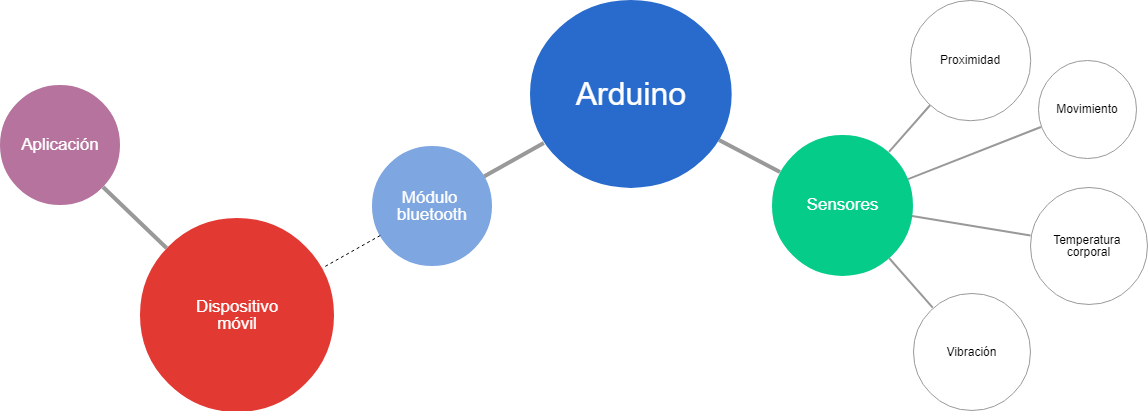
\includegraphics[width=1\linewidth]{esquemageneral}
				\caption{Esquema general}
				\label{esquemageneral}
			\end{figure}

		\subsection{Arduino}

			Gracias al avance tecnológico, hoy en día podemos contar con dispositivos pre-diseñados que nos ayudan en los desarrollos posteriores ahorrando mucho tiempo y costos. Es así que Arduino, una empresa italiana, desarrolló una plaqueta que cumple la funcion de un micro-controlador programable, adaptandosé a lo largo de los años hacia distintos módulos y tecnologías o posibilidades que se pudieran aplicar al mismo. Gracias a la plaqueta Arduino y su programación interna a medida según se requiera, se pueden conectar varios sensores que serán mencionados a continuación para la obtención de los datos relevantes, y hacer uso de ellos según se desee. 
			Como se puede apreciar en la \textbf{Figura \ref{arduino-mega}}, se estará utilizando la versión Mega 2560 de Arduino, en donde los distintos módulos requeridos serán conectados a través de sus pines de entrada y salida (analógico y/o digital) que se puden observar.

			\begin{figure}
				\centering
				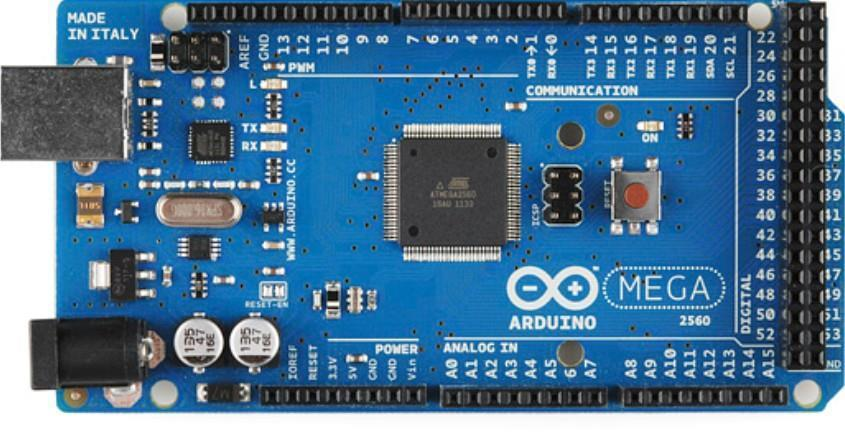
\includegraphics[width=1\linewidth]{arduino-mega}
				\caption{Arduino MEGA 2560}
				\label{arduino-mega}
			\end{figure}

		\subsection{Sensores}

			\subsubsection{Módulo sensor de proximidad (\textbf{IR FC-51})}

			El sensor representado en la \textbf{Figura \ref{arduino-modulo-proximidad}} detecta interposición de algun objeto entre una distancia pre-configurada y el mismo (sin contacto, entre una distancia de 2 cm a 30 cm, y con un ángulo de detección de 35º). La utilidad de éste sensor se verá reflejada ante la necesidad de detectar si el bebé se encuentra dentro del área de estudio de donde se obtendrían los datos de los otros sensores incorporados, o si el sistema debiera descartar los datos obtenidos o mismo desactivar los sensores ante la ausencia del bebé en el área e informar hacia la aplicación móvil. El sensor funciona mediante la transmisión de ondas o impulsos infrarrojos los cuales son transmitidos hacia la dirección aproximada donde se dirige el mismo, y recepciona las ondas que rebotan en determinados objetos en caso de haberlos, es decir que trabaja sobre la reflexión de luz infrarroja. El presente módulo cuenta con un potenciómetro el cual regula la sensibilidad de las detecciones, pudiéndose traducirse como sensibilidad de distancia de objetos. 

				\begin{figure}
					\centering
					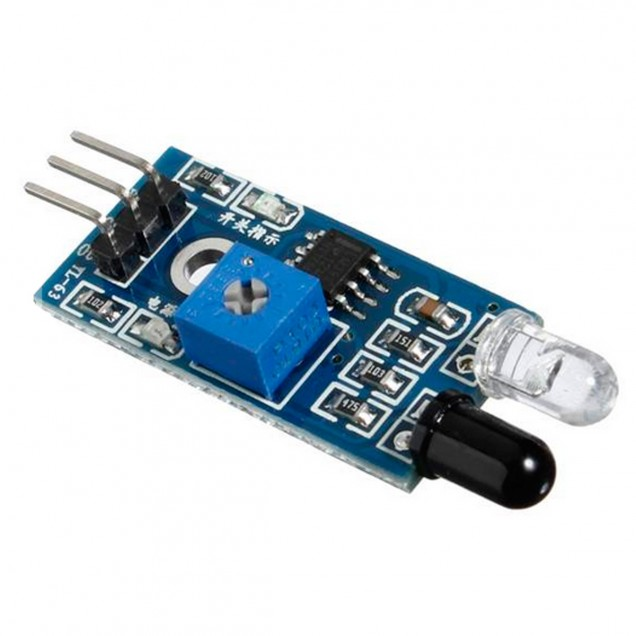
\includegraphics[width=0.6\linewidth]{arduino-modulo-proximidad}
					\caption{Módulo de proximidad infrarrojo IR FC-51 para Arduino}
					\label{arduino-modulo-proximidad}
				\end{figure}

			\subsubsection{Módulo sensor de temperatura direccional (\textbf{MLX90614})}
			
			Es un sensor de temperatura direccional sin contacto y con incidencia hacia un cierto rango de distancia entre el objeto observado y el sensor mismo. El sensor de temperatura mencionado funciona bajo un receptor de luz infrarroja a través de las radiaciones recibidas (según la ley de Stefan-Boltzmann, todo objeto por encima del cero absoluto emite radiación cuyo espectro es proporcional a su temperatura). Una imagen del sensor mencionado se puede observar en la \textbf{Figura \ref{arduino-modulo-temperatura}} y será el encargado de obtener la temperatura corporal del lactante al direccionarse hacia donde se presupone va a estar posicionada la cabeza del bebé, de forma tal que el indicador obtenido por dicho sensor sea lo más certero posible.

				\begin{figure}
					\centering
					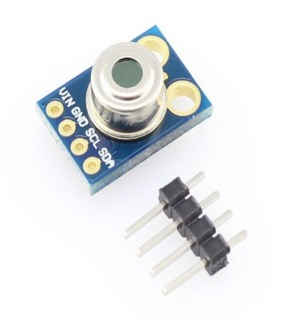
\includegraphics[width=0.6\linewidth]{arduino-modulo-temperatura}
					\caption{Módulo de temperatura direccional MLX90614 para Arduino}
					\label{arduino-modulo-temperatura}
				\end{figure}

			\subsubsection{Módulo sensor de vibración (\textbf{AA2758})}
			
			Sensor analógico que se basa en un mecanísmo de cerámica entre placas metálicas, comunmente denominado piezoeléctrico, el cual reacciona ante vibraciones generando señales eléctricas que son obtenidas y enviadas a la placa Arduino para su posterior manipulación o interpretación. El objetivo de éste sensor es el de obtener movimientos y vibraciones que sean localizados por debajo del bebé a través de una red de piezoeléctricos. Con la sensibilidad adecuada y la interpretación de los datos obtenidos se puede realizar un control sobre la respiración del bebé ante la variación de presión por el movimiento toráxico que ésto implica. En la \textbf{Figura \ref{arduino-modulo-vibracion}} se observa el módulo correspondiente y el piezoeléctrico conectado al mismo.

				\begin{figure}
					\centering
					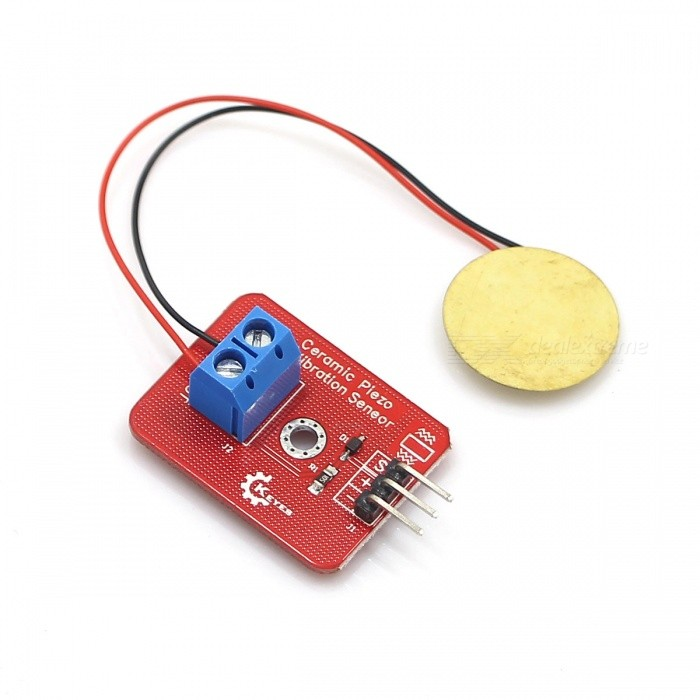
\includegraphics[width=0.6\linewidth]{arduino-modulo-vibracion}
					\caption{Módulo sensor de vibración AA2758 para Arduino}
					\label{arduino-modulo-vibracion}
				\end{figure}

			\subsubsection{Módulo sensor de movimiento (\textbf{HC-SR501})}
			
			Módulo el cual integra un sensor PIR (Passive Infrared), generalmente utilizado para sistemas de alarma en la detección de movimiento. Se basan en la medición de la radiación infrarroja en distintos campos, cuando detectan variaciones de radiación entre los campos significa que hubo algún movimiento en su campo de visión. La principal función de éste módulo radica en medir la cantidad de movimiento durante el sueño del lactante y detectar cuales son los horarios en que podría despertarse durante la noche. Además indicaría cuáles son aquellos ciclos en donde el bebé pudo haberse movido de alguna manera ocacionando una modificación en la postura en la que fue colocado y pudiendo obtruír las vías respiratorias. En la \textbf{Figura \ref{arduino-modulo-movimiento}} se puede observar el módulo sensor de detección de movimiento.

				\begin{figure}
					\centering
					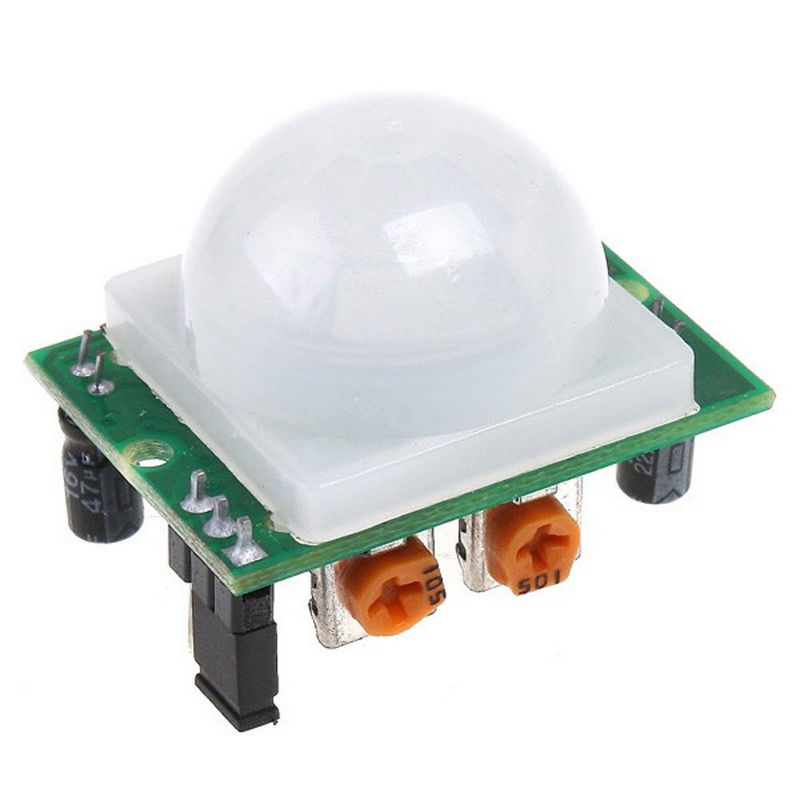
\includegraphics[width=0.6\linewidth]{arduino-modulo-movimiento}
					\caption{Módulo sensor de movimiento HC-SR501 para Arduino}
					\label{arduino-modulo-movimiento}
				\end{figure}

		\subsection{Módulo de comunicación (\textbf{HC-06})}

		Es otro de los módulos más importantes que tiene el sistema ya que es el encargado de comunicarse inalambricamente con el dispositivo móvil, cuya aplicación está instalada, y así transmitir datos, visualizar indicadores y alertar ante cualquier incidente que pudiese ocurrir que ponga en riesgo la vida del bebé. El módulo mencionado realiza una conexión punto a punto entre la plaqueta Arduina que recolecta toda la información y el dispositivo móvil (teléfono celular o tablet) que tiene la aplicación. Es importante destacar que éste módulo trabaja con una tecnología de bluetooth tradicional y no BLE, con lo que representa una incompatibilidad con los dispositivos de Apple. En la \textbf{Figura \ref{arduino-modulo-bluetooth}} se puede observar el módulo de comunicación bluetooth mencionado.

			\begin{figure}
				\centering
				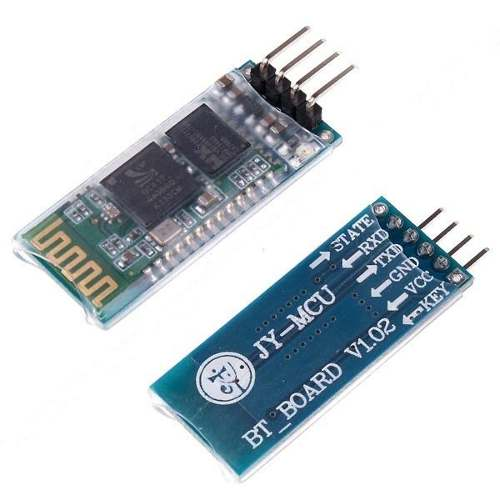
\includegraphics[width=0.6\linewidth]{arduino-modulo-bluetooth}
				\caption{Módulo de comunicación bluetooth HC-06}
				\label{arduino-modulo-bluetooth}
			\end{figure}

% Se pueden poner referencias a sitios web?

		\subsection{Aplicación móvil}
		
			El uso de los dispositivos móviles es algo que ya forma parte de nuestra cultura diaria, y es por ello que el proyecto presentado tiene relacion a la conectividad móvil, ya que es posible hacer llegar la informacion leida por los sensores a dispositivos móviles, permitiendo estar en contacto permanente con el estado de las diferentes variables ambientales que rodean y afectan al bebé, pudiendo inferir en el bienestar del mismo. Las alertas o notificaciones emitidas por la aplicación son producto de parámetros que varían a través del tiempo, identificando los cambios abruptos de los mismos indicando algun cambio de estado. 
			
			En este proyecto la aplicación móvil estará desarrollada tanto para la plataforma Android como iOS, pero cabe destacar que la compatibilidad del hardware de las plataformas mencionadas y el módulo de conectividad Bluetooth utilizada solamente es viable con dispositivos Android, ya que los dispositivos iOS utilizan otro tipo de tecnología conocida como BLE (Bluetooth Low Energy).
			El desarrollo del aplicativo estará basado sobre Ionic, el cual es un framework diseñado para el desarrollo de aplicaciones móviles híbridas, el cual se basa en Angular, Typescript, Javascript, CSS3 y HTML5. El concepto principal se basa en la traducción gráfica de todos los componentes visualizados en cada dispositivo móvil dependiendo la plataforma en la cual se encuentre, ya sea para Android o para iOS, cada componente utilizado tiene su representación gráfica acorde a la plataforma.
			Uno de los principales pilares que tiene Ionic es el de incorporar las librerías de Apache Cordova, la cual contiene toda la lógica, o motor principal, para traducir el código desarrollado independiente por cada plataforma. Es decir, Cordova contiene los desarrollos individuales, algunos desarrollados oficialmente y otros por grupos de desarrolladores de la comunidad que hacen su aporte, de los plugins que hacen a la funcionalidad de cada módulo del sistema operativo en cuestión. En la \textbf{Figura \ref{ionic-angular-cordova}} se puede observar cómo interactúan los distintos componentes que hacen al desarrollo de la plataforma final distribuida para cada sistema operativo.


			\begin{figure}
				\centering
				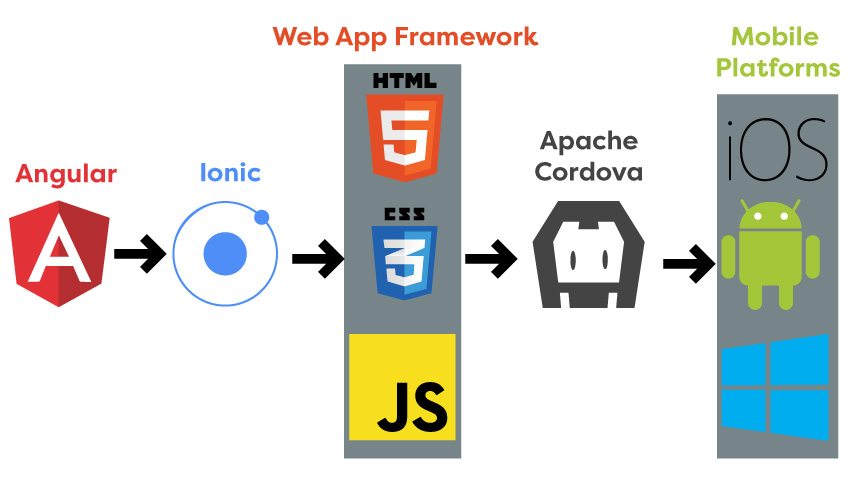
\includegraphics[width=1\linewidth]{ionic-angular-cordova}
				\caption{Esquema de arquitecturas Ionic - Angular - Cordova}
				\label{ionic-angular-cordova}
			\end{figure}

			En lo que respecta al desarrollo híbrido, el aplicativo final para cada plataforma, se traduce como un navegador web incorporado el cual es visualizado por el usuario final. Es por ello que el desarrollo principal está hecho sobre plataformas web. En la \textbf{Figura \ref{ionic-angular-cordova-webview}} se observa el componente WebView que interpreta los recursos incorporados y los lenguajes HTML, CSS y Javascript, dicho componente es el que simula un navegador web dentro del aplicativo final.

			\begin{figure}
				\centering
				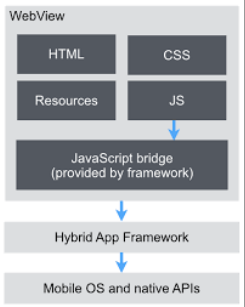
\includegraphics[width=0.6\linewidth]{ionic-angular-cordova-webview}
				\caption{Componentes internos Cordova}
				\label{ionic-angular-cordova-webview}
			\end{figure}
			

%%%%%%%%%%%%%%%%%%%%%%%%%%%%%%%%%%%%


	\section{Desarrollo}
		
%		El dispositivo que realizará la función de monitoreo al lactante se concentra en un hardware que no es invasivo para el mismo. Los sistemas de medición que se aplican, es decir, los diferentes sensores que toman datos del lactante, no deben tener contacto directo con el mismo. De esta forma la forma y estructura de funcionamiento será lo más normal y natural cotidiano que se encuentra día tras día en los hogares. En la investigación previa a la realización del presente documento se han encontrado diferentes sistemas ya creados a nivel mundial, los cuales algunos de ellos requieren algún tipo de contacto exclusivo con la piel del bebé, como por ejemplo en aquellos dispositivos que son incorporados en la vestimenta, obligando a los padres y/o tutores a tomar ciertas medidas previas a la colocación del bebé en la cuna las cuales se pueden llegar a tornar medias tediosas o directamente ser rechazadas por los responsables al ser un tanto invasivas. También en la investigación se han encontrado algunos dispositivos los cuales no tienen contacto directo con el lactante, los cuales fueron tomados de ejemplo y estudio para generar el dispositivo actual con distintos valores agregados.
%
%ARDUINO IDE, codigo y librerias.
%
%			\begin{figure}
%				\centering
%				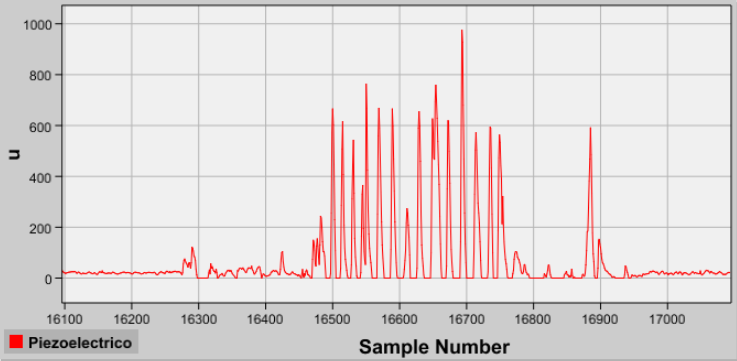
\includegraphics[width=1\linewidth]{piezo}
%				\caption{Sensor de vibración}
%				\label{piezo}
%			\end{figure}
%
%			\begin{figure}
%				\centering
%				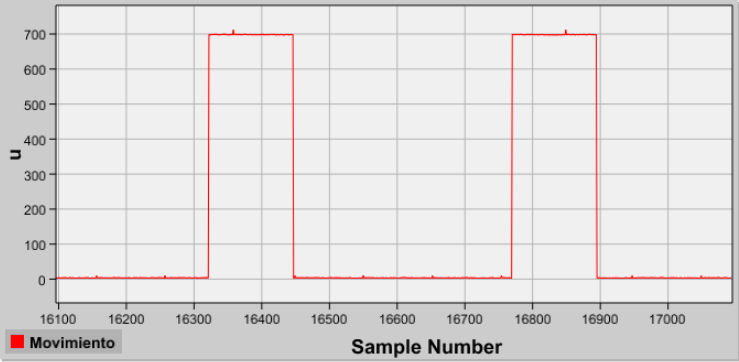
\includegraphics[width=1\linewidth]{movimiento}
%				\caption{Detector de movimiento}
%				\label{movimiento}
%			\end{figure}
%
%			\begin{figure}
%				\centering
%				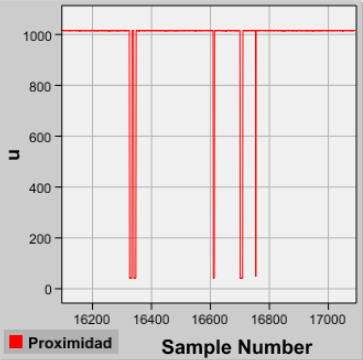
\includegraphics[width=1\linewidth]{proximidad}
%				\caption{Sensor de proximidad}
%				\label{proximidad}
%			\end{figure}
%
%			\begin{figure}
%				\centering
%				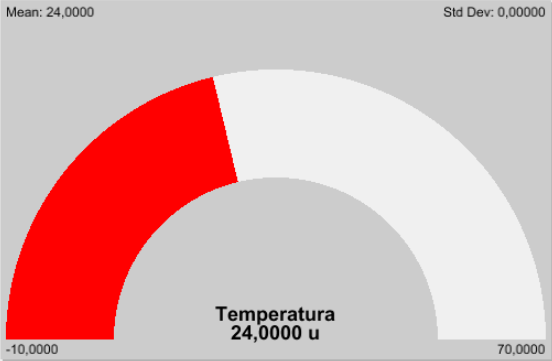
\includegraphics[width=1\linewidth]{temperatura}
%				\caption{Sensor de temperatura}
%				\label{temperatura}
%			\end{figure}
%			
%			\begin{figure}
%				\centering
%				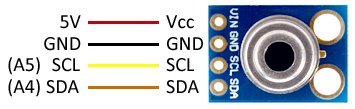
\includegraphics[width=1\linewidth]{arduino-modulo-temperatura-pines}
%				\caption{Módulo de temperatura direccional MLX90614 para Arduino}
%				\label{arduino-modulo-temperatura-pines}
%			\end{figure}

		\subsection{Metodología}
			
%			La metodología implementada para la solución
			
		\subsection{Sistemas de medición}
		
		\subsection{Visualización y alertas}
	
	\section{Conclusión}

		\subsection{Mejoras}

%Incubadoras
%Wifi
%Luz: lux vs lumenes. A flux of 1000 lumens, concentrated into an area of 1 square metre, lights up that square metre with an illuminance of 1000 lux. However, the same 1000 lumens, spread out over 10 square metres, produces a dimmer illuminance of only 100 lux. https://en.wikipedia.org/wiki/Lux
%Temperatura y Humedad
%Sonido
%Gases (monóxido de carbono, gas butano y humos): 

		\subsection{Lecciones aprendidas para trabajos futuros}

	\section{Investigación bibliográfica}
		\nocite{*}
	
		\cite{garcia2008sindrome} - Trabajo de revisión sobre las causas, factores de riesgo, epidemología y recomendaciones sobre el SMSL por Felipa Elena García García, Especialista de II Grado en Pediatría. Profesora Auxiliar. Hospital Pediátrico Docente "Juan M. Márquez". La Habana, Cuba.

		\cite{subita2000nuevas} - Nuevas recomendaciones para evitar el SMSL realizadas por un trabajo de grupo de investigación de muertes súbitas.

		\cite{silva2008device} - Dispositivo para el monitoreo de la respiración tanto en humanos como en animales, el mismo contiene un acelerómetro y un microprocesador para la detección del movimiento. Trabajo desarrollado por Carlos Silva.

		\cite{hafner2007non} - Utilización de un baby monitor y un dispositivo radar doopler para el monitoreo de la actividad cardiopulmonar. Trabajo desarrollado por Noah Hafner, Isar Mostafanezhad, Victor M. Lubecke, Olga Boric-Lubecke, y Anders Host-Madsen.

		\cite{brady2005garment} - Monitoreo del ritmo de respiración basado en prendas de vestir en un diagnóstico de 10 minutos. Desarrollado por Sarah Brady, Lucy E Dunne, Richard Tynan, Dermot Diamond, Barry Smyth, y Gregory M.P. O’Hare en la Universidad de la Ciudad de Dublin.

		\cite{scanlon1996sudden} - Monitor de actividad acústica y movimiento (por ejemplo respiración o latidos). También cuenta conun estimulador. Trabajo desarrollado por Michael Scanlon.

		\cite{kim1996sudden} - Monitor de desaturacion oxigeno y movimiento para prevenir el SMSL con sistema de alertas incluido ante el cambio de indicadores. Trabajo desarrollado por Bill H. Kim.

		\cite{teodorescu2000respiration} - Trabajo realizado por Horia-Nicolai Teodorescu y Daniel J. Mlynek, el cual consiste en un sistema de monitoreo de respiración y movimiento en infantes, los datos son recolectados a través de una plataforma con un acelerómetro, también con alarmas incorporadas.

		\cite{christian1999apparatus} - Es un trabajo desarrollado por Christian P. von der Heyde, el cual consiste en un sistema para prevenir el SMSL por asfixia debida al contenido de monóxido de carbono en aire.

		\cite{lee2012baby} - Trabajo de Taek Kyu LEE y Min Soo Han, el cual consiste en un sistema de monitoreo de bebés remoto con un dispositivo incorporado en el abdomen del lactante en forma de cinturón. Monitorea el ritmo de respiración y la orientación del cuerpo.

		\cite{broussard2002baby} - Es un trabajo realizado por Rose Broussard y Johnny Broussard, el cual consiste en una manta inteligente posicionada por debajo del bebé para monitorear la distribución del peso. Contiene un sistema de alarma el cual se activa si el peso no está distribuído dentro de un rango en la misma, indicando el movimiento del lactante.

		\cite{hernandez2017deteccion} - Se basa en un trabajo de investigación sobre los métodos de detección de la respiración de forma no invasiva hacia el sujeto en cuestión, mediante un imán inductor conectado a un microcontrolador. Trabajo realizado por A. Hernández, E. Sifuentes, J. Cota, y R. González Landaeta.

		\cite{esquiroz2017diseno} - Diseño, fabricación y caracterización de un sistema de
detección de monóxido de carbono en la respiración humana. Trabajo realizado por Aitor Esquíroz Olcoz.

		\cite{min2010noncontact} - Es un sensor de proximidad ultrasónico, el cual obtiene la información de la respiración a través de un lazo incorporado en la cintura. Trabajo realizado por Se Dong Min, Jin Kwon Kim, y Hang Sik Shin, miembros y estudiantes de IEEE.
Yong Hyeon Yun, Student Member, IEEE, Chung Keun Lee, Student Member, IEEE, and Myoungho Lee.

		\cite{lindberg1996estimation} - Estimación del ritmo de respiración y concentración de oxígeno. Trabajo desarrollado por C. F. Lindberg y B. Carlsson.

		\bibliographystyle{IEEEtran}	
		\bibliography{bibliografia}
	
\end{document}


%TEXTO DE EJEMPLO DEL PROFESOR

%\textbf{En un lugar de la Mancha}

%\section{...}
%\subsection{...}
%\subsubsection{...}
%\paragraph{...}
%\subparagraph{...}

%	\begin{table}
%		\centering
%		\caption{Mi primera tabla}
%		\begin{tabular}{|l|l|l|l|l|l|l|l|l|}
%			\hline
%			Muerte súbita & 1991 & 1992 & 1993 & 1994 & 1995 & 1996 & 1997 & 1998 \\
%			\hline
%			0-365 días & 552 & 516 & 506 & 484 & 500 & 467 & 383 & 417 \\
%			\hline
%			28-365 días & 437 & 397 & 380 & 361 & 393 & 378 & 301 & 320 \\
%			\hline
%			Recién nacidos vivos & 694.746 & 678.761 & 667.518 & 667.787 & 658.735 & 675.437 & 692.537 & 683.301 \\
%			\hline
%			Tasa de mortalidad posneonatal por SMSL & 0.63 & 0.58 & 0.57 & 0.54 & 0.60 & 0.56 & 0.43 & 0.47 \\
%			\hline
%			Tasa de mortalidad posneonatal & 9.30 & 8.70 & 8.40 & 7.60 & 8.10 & 7.90 & 7.00 & 7.40 \\
%			\hline
%		\end{tabular}
%		\label{tab.tabla1}
%	\end{table}
	
	%Como se presenta en la figura \ref{gatofeliz} el gato naranja está feliz de vivir.
	
	%\begin{table}
	%	\centering
	%	\caption{Mi primera tabla}
	%	\begin{tabular}{|l|p{4cm}|l|r|}
	%		\hline
	%		uno & dos & tres & ddddcuatro \\
	%		\hline
	%		one & competencia con el cura de su lugar (que era hombre docto graduado en Sigüenza & threeddddd & four \\
	%		\hline
	%	\end{tabular}
	%	\label{tab.tabla1}
	%\end{table}
	
%	Tuvo muchas veces en la tabla \ref{tab.tabla1} competencia con el cura de su lugar (que era hombre docto graduado en Sigüenza), sobre cuál había sido mejor caballero, Palmerín de Inglaterra o Amadís de Gaula; mas maese Nicolás, barbero del mismo pueblo, decía que ninguno llegaba al caballero del Febo, y que si alguno se le podía comparar, era don Galaor, hermano de Amadís de Gaula, porque tenía muy acomodada condición para todo; que no era caballero melindroso, ni tan llorón como su hermano, y que en lo de la valentía no le iba en zaga.
%	
%	En la sección \ref{sec.desarrollo} se presenta el trabajo realizado.
%	
%	\section{Desarrollo}\label{sec.desarrollo}
%	
%	En resolución, él se enfrascó tanto en su lectura, que se le pasaban las noches leyendo de claro en claro, y los días de turbio en turbio, y así, del poco dormir y del mucho leer, se le secó el cerebro, de manera que vino a perder el juicio. Llenósele la fantasía de todo aquello que leía en los libros, así de encantamientos, como de pendencias, batallas, desafíos, heridas, requiebros, amores, tormentas y disparates imposibles, y asentósele de tal modo en la imaginación que era verdad toda aquella máquina de aquellas soñadas invenciones que leía, que para él no había otra historia más cierta en el mundo.
%	\\
%	\\	%salto de linea
%	\\
%	\newpage
%	
%	Enumeradores:
%	
%	\begin{enumerate}
%		\item Linea uno
%		\item Linea dos
%		\begin{enumerate}
%			\item dos.uno
%			\item dos.dos
%		\end{enumerate}
%		\item Linea tres
%	\end{enumerate}
%	
%	Viñetas:
%	
%	\begin{itemize}
%		\item Primer item
%		\item Segundo item
%			\begin{itemize}
%				\item Segundo.primer item
%				\item Segundo.segundo item
%			\end{itemize}
%		\item Tercer item
%	\end{itemize}
%	
%	Descripciones:
%	
%	\begin{description}
%		\item[Clase] Es una representación de metodos y atributos que 
%		\item[Objeto] Es una instancia de la clase
%	\end{description}
%	
%	Decía él, que el Cid Ruy Díaz había sido muy buen caballero; pero que no tenía que ver con el caballero de la ardiente espada, que de sólo un revés había partido por medio dos fieros y descomunales gigantes. Mejor estaba con Bernardo del Carpio, porque en Roncesvalle había muerto a Roldán el encantado, valiéndose de la industria de Hércules, cuando ahogó a Anteo, el hijo de la Tierra, entre los brazos. Decía mucho bien del gigante Morgante, porque con ser de aquella generación gigantesca, que todos son soberbios y descomedidos, él solo era afable y bien criado; pero sobre todos estaba bien con Reinaldos de Montalbán, y más cuando le veía salir de su castillo y robar cuantos topaba, y cuando en Allende robó aquel ídolo de Mahoma, que era todo de oro, según dice su historia. Diera él, por dar una mano de coces al traidor de Galalón, al ama que tenía y aun a su sobrina de añadidura.
%	
%	\begin{equation}\label{eq.int}
%		f(x)= \int_{0}^{\infty} x^2 dx 
%	\end{equation}
%	
%	\begin{equation}\label{eq.int2}
%	f(x)= \int_{0}^{\infty} x^2 dx 
%	\end{equation}
%	
%	\begin{equation}\label{eq.suma}
%		f(x)= \sum_{1}^{n} \frac{1}{x} 
%	\end{equation}
%	
